% !TEX encoding = UTF-8 Unicode
% -*- coding: UTF-8; -*-
% vim: set fenc=utf-8

\section{Existující řešení}\label{sec:existujícíŘešení}
V této sekci představuji již existující nástroje pro kolaborativní editaci textů a prozradím, který algoritmus pro sdílení textů používají.

\subsection{Apache Wave}\label{subsec:apacheWave}
Apache Wave je pokračováním produktu Google Wave od společnosti Google po jeho ukončení.
V lednu roku 2018 byl jeho vývoj pod záštitou Apache Foundation ukončen a není v něm již pokračováno.~\cite{wave:apache}

Jedná se o serverové řešení komunikace ve skutečném čase napsané v jazyce Java, které obsahuje implementaci protokolu Wave Federation.
Protokol Wave Federation byl navržen jako rozšíření algoritmu \gls{OT} (více o algoritmu v~\ref{subsec:operacniTransformace}) společností Google a zasloužil se o důležité vylepšení v podobě potvrzování každé přijaté operace serverem.~\cite{wave:apache},~\cite{wave:google}
Projekt dnes není prakticky nasaditelný (nevyšla žádná stabilní verze), ale je považován za důležitý krok k rozšíření kolaborativní editace~\cite{ot:codecommit}.

\subsection{Google Docs}\label{subsec:googleDocs}
Google Docs je textový procesor, který je spolu s dalšími kancelářskými aplikacemi součástí služby Google Drive od společnosti Google.
Jedná se o editor typu \gls{WYSIWYG} podobný ostatním kancelářským textovým procesorům (jako je například Microsoft Word, OpenOffice Writer a další).~\cite{docs:top10}

Google Docs využívá Google Apps API, které je také postaveno nad algoritmem \gls{OT} (více o algoritmu v~\ref{subsec:operacniTransformace})~\cite{docs:conflict} a to včetně vylepšení, se kterým přišel Google při vývoji Google Wave~\cite{docs:appsConf}.

\begin{figure}[ht]
    \centering
    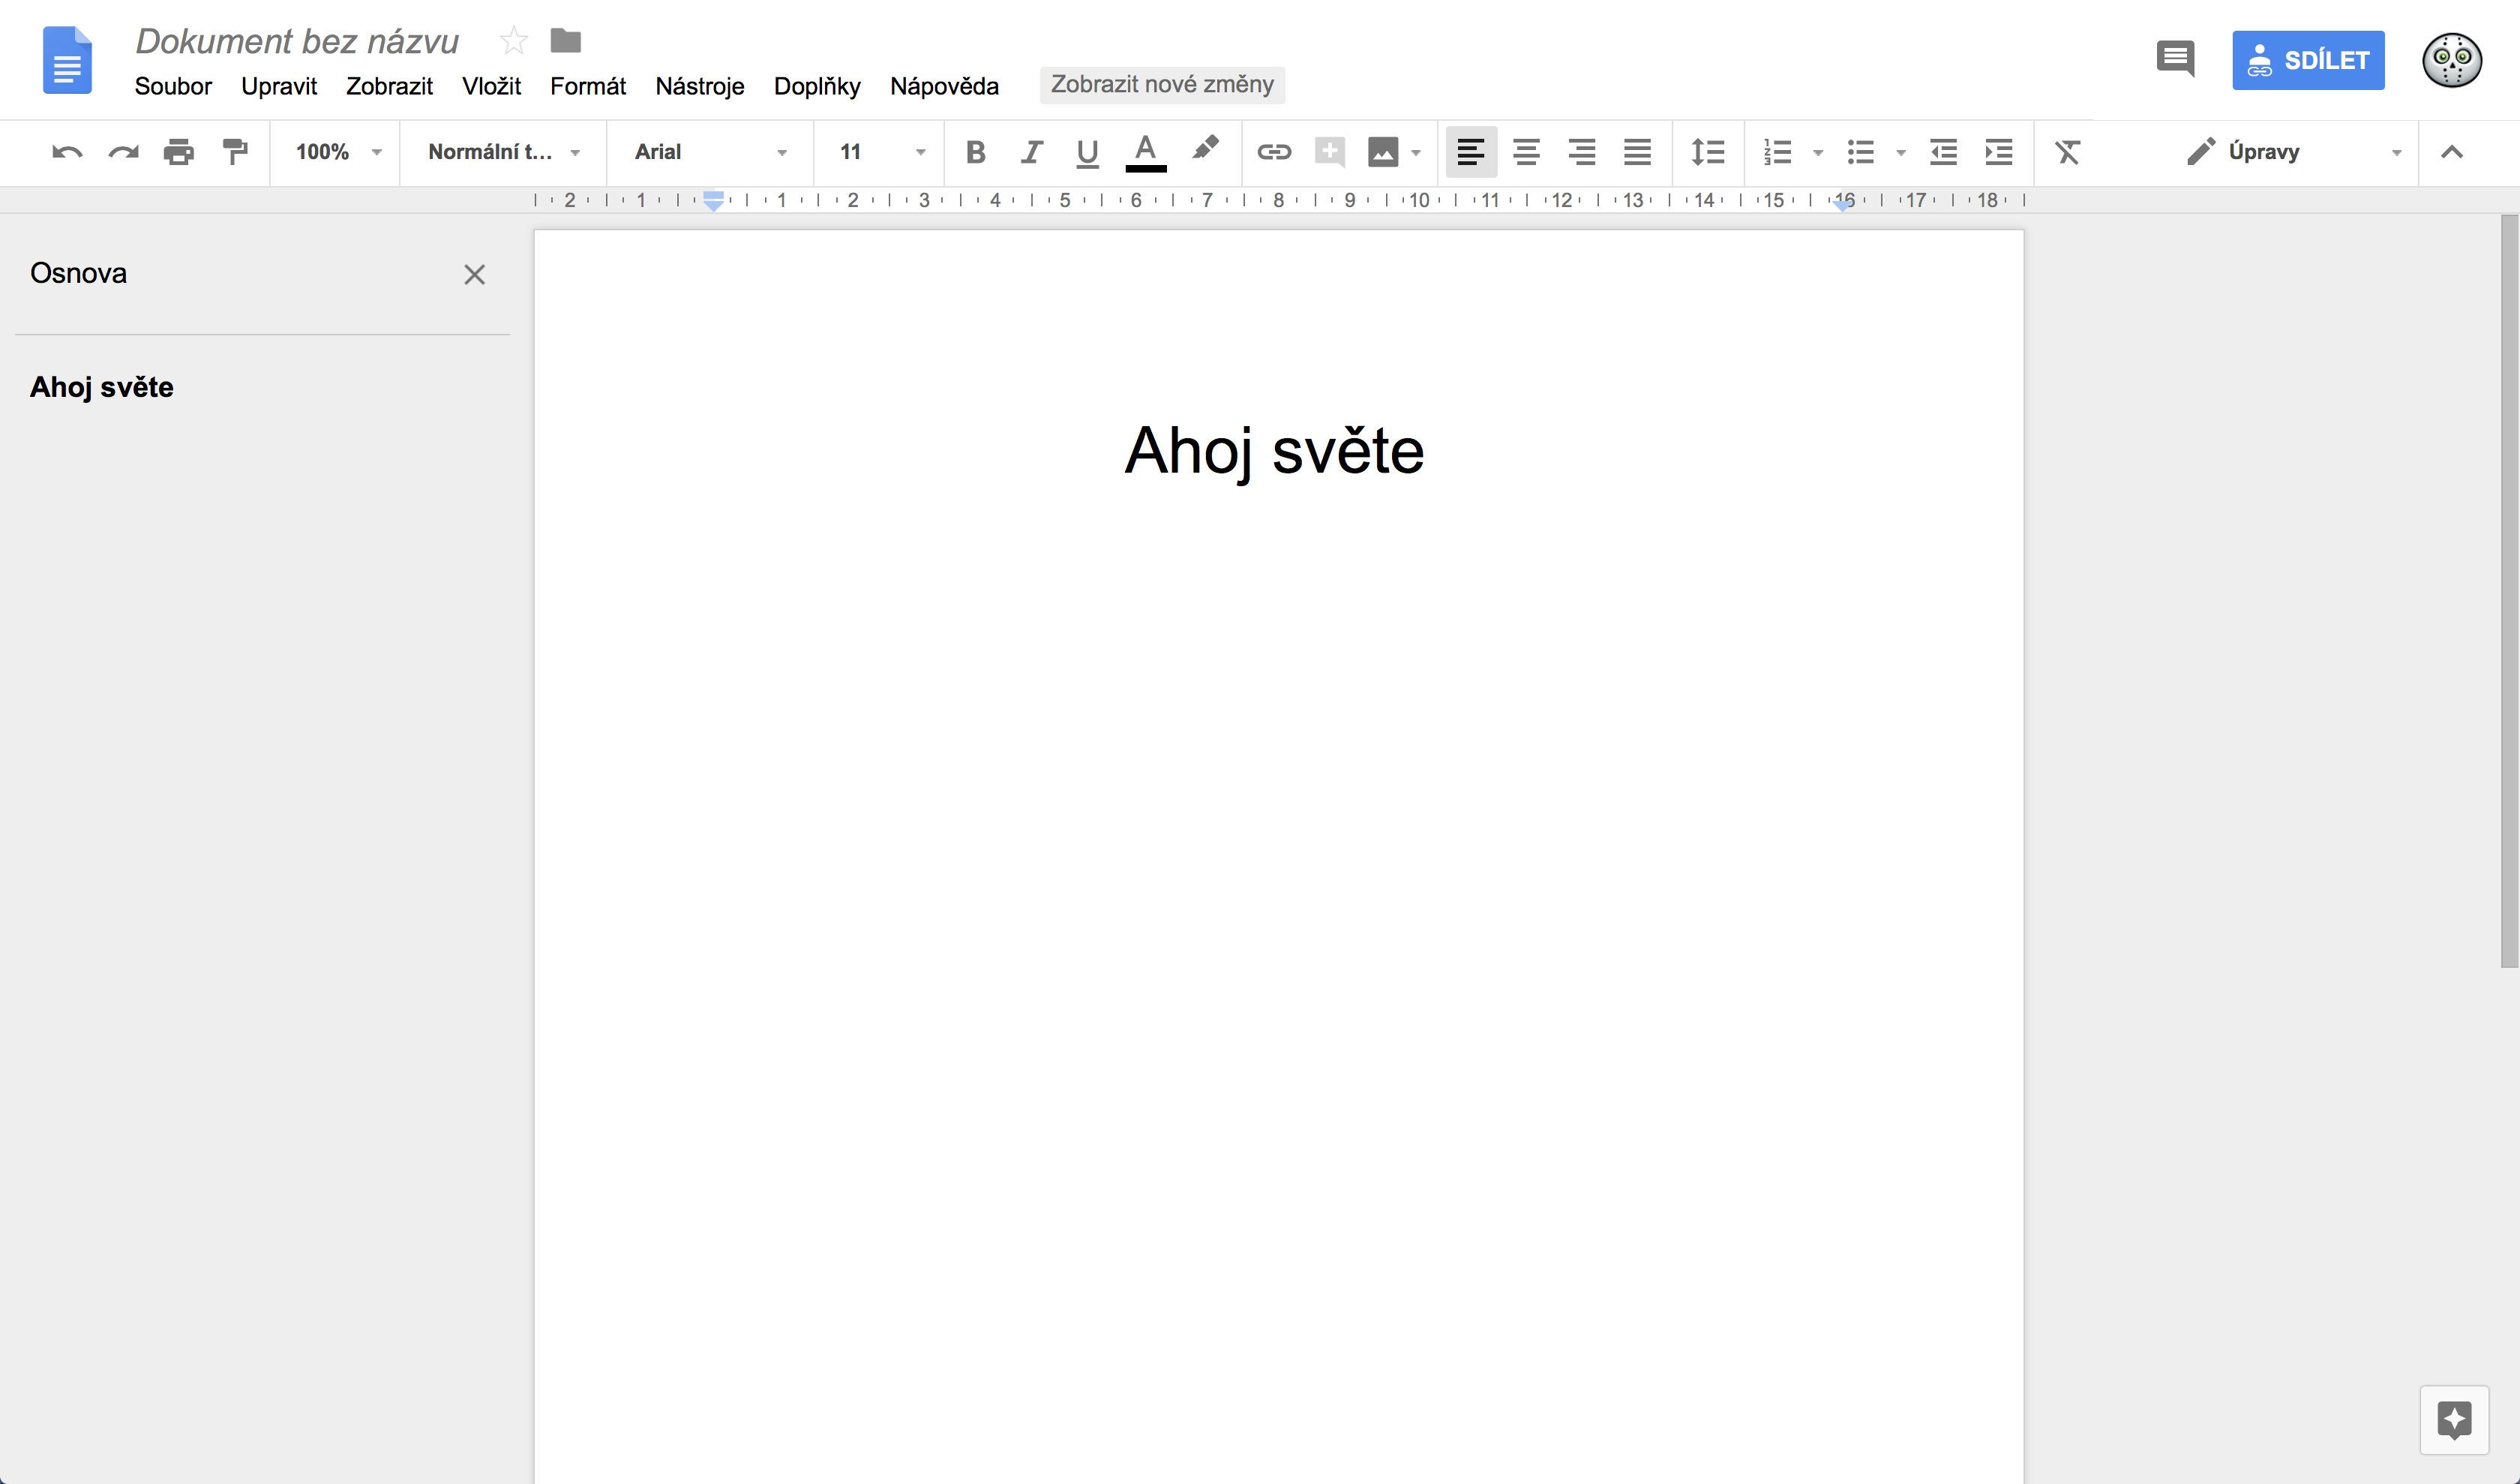
\includegraphics[width=\textwidth]{partials/analyza/googleDocs}
    \caption{Ukázka aplikace Google Docs}\label{fig:googleDocs}
\end{figure}

\subsection{Etherpad}\label{subsec:etherpad}

EtherPad jako webová služba pro kolaborativní editaci textů byla odkoupena společností Google roku 2009 za účelem integrace do tehdejší služby Google Wave~\cite{etherpad:acquired}.
Google poté zveřejnil zdrojové kódy služby a vznikl tak projekt Etherpad, webový textový procesor s otevřeným zdrojovým kódem~\cite{etherpad:openSource}.

Etherpad byl od zveřejnění otevřeného kódu přepsán z jazyka Scala do JavaScriptu~(více o JavaScriptu v~\ref{subsec:javascript}) pro serverové prostředí NodeJS~(více o NodeJS v~\ref{subsec:nodejs}), ale původní synchronizační knihovna nazývaná EasySync zůstává nadále stejná~\cite{etherpad:newgithub},~\cite{etherpad:easySync}.
Knihovna EasySync (a tím tedy i Etherpad samotný) využívá principy algoritmu \gls{OT} (více o algoritmu v~\ref{subsec:operacniTransformace}) a to včetně vylepšení ve formě čekání klienta po odeslání operace na potvrzení od serveru~\cite{etherpad:easySync}.
Dnes existuje množství nejrůznějších zásuvných modulů, které rozšiřují možnosti nástroje Etherpad a to i včetně modulu pro komunikaci pomocí \gls{WebRTC}, protokol umožňující implementaci audio, či video hovorů přímo ve webovém prohlížeči.~\cite{etherpad:plugins}.

\begin{figure}[ht]
    \centering
    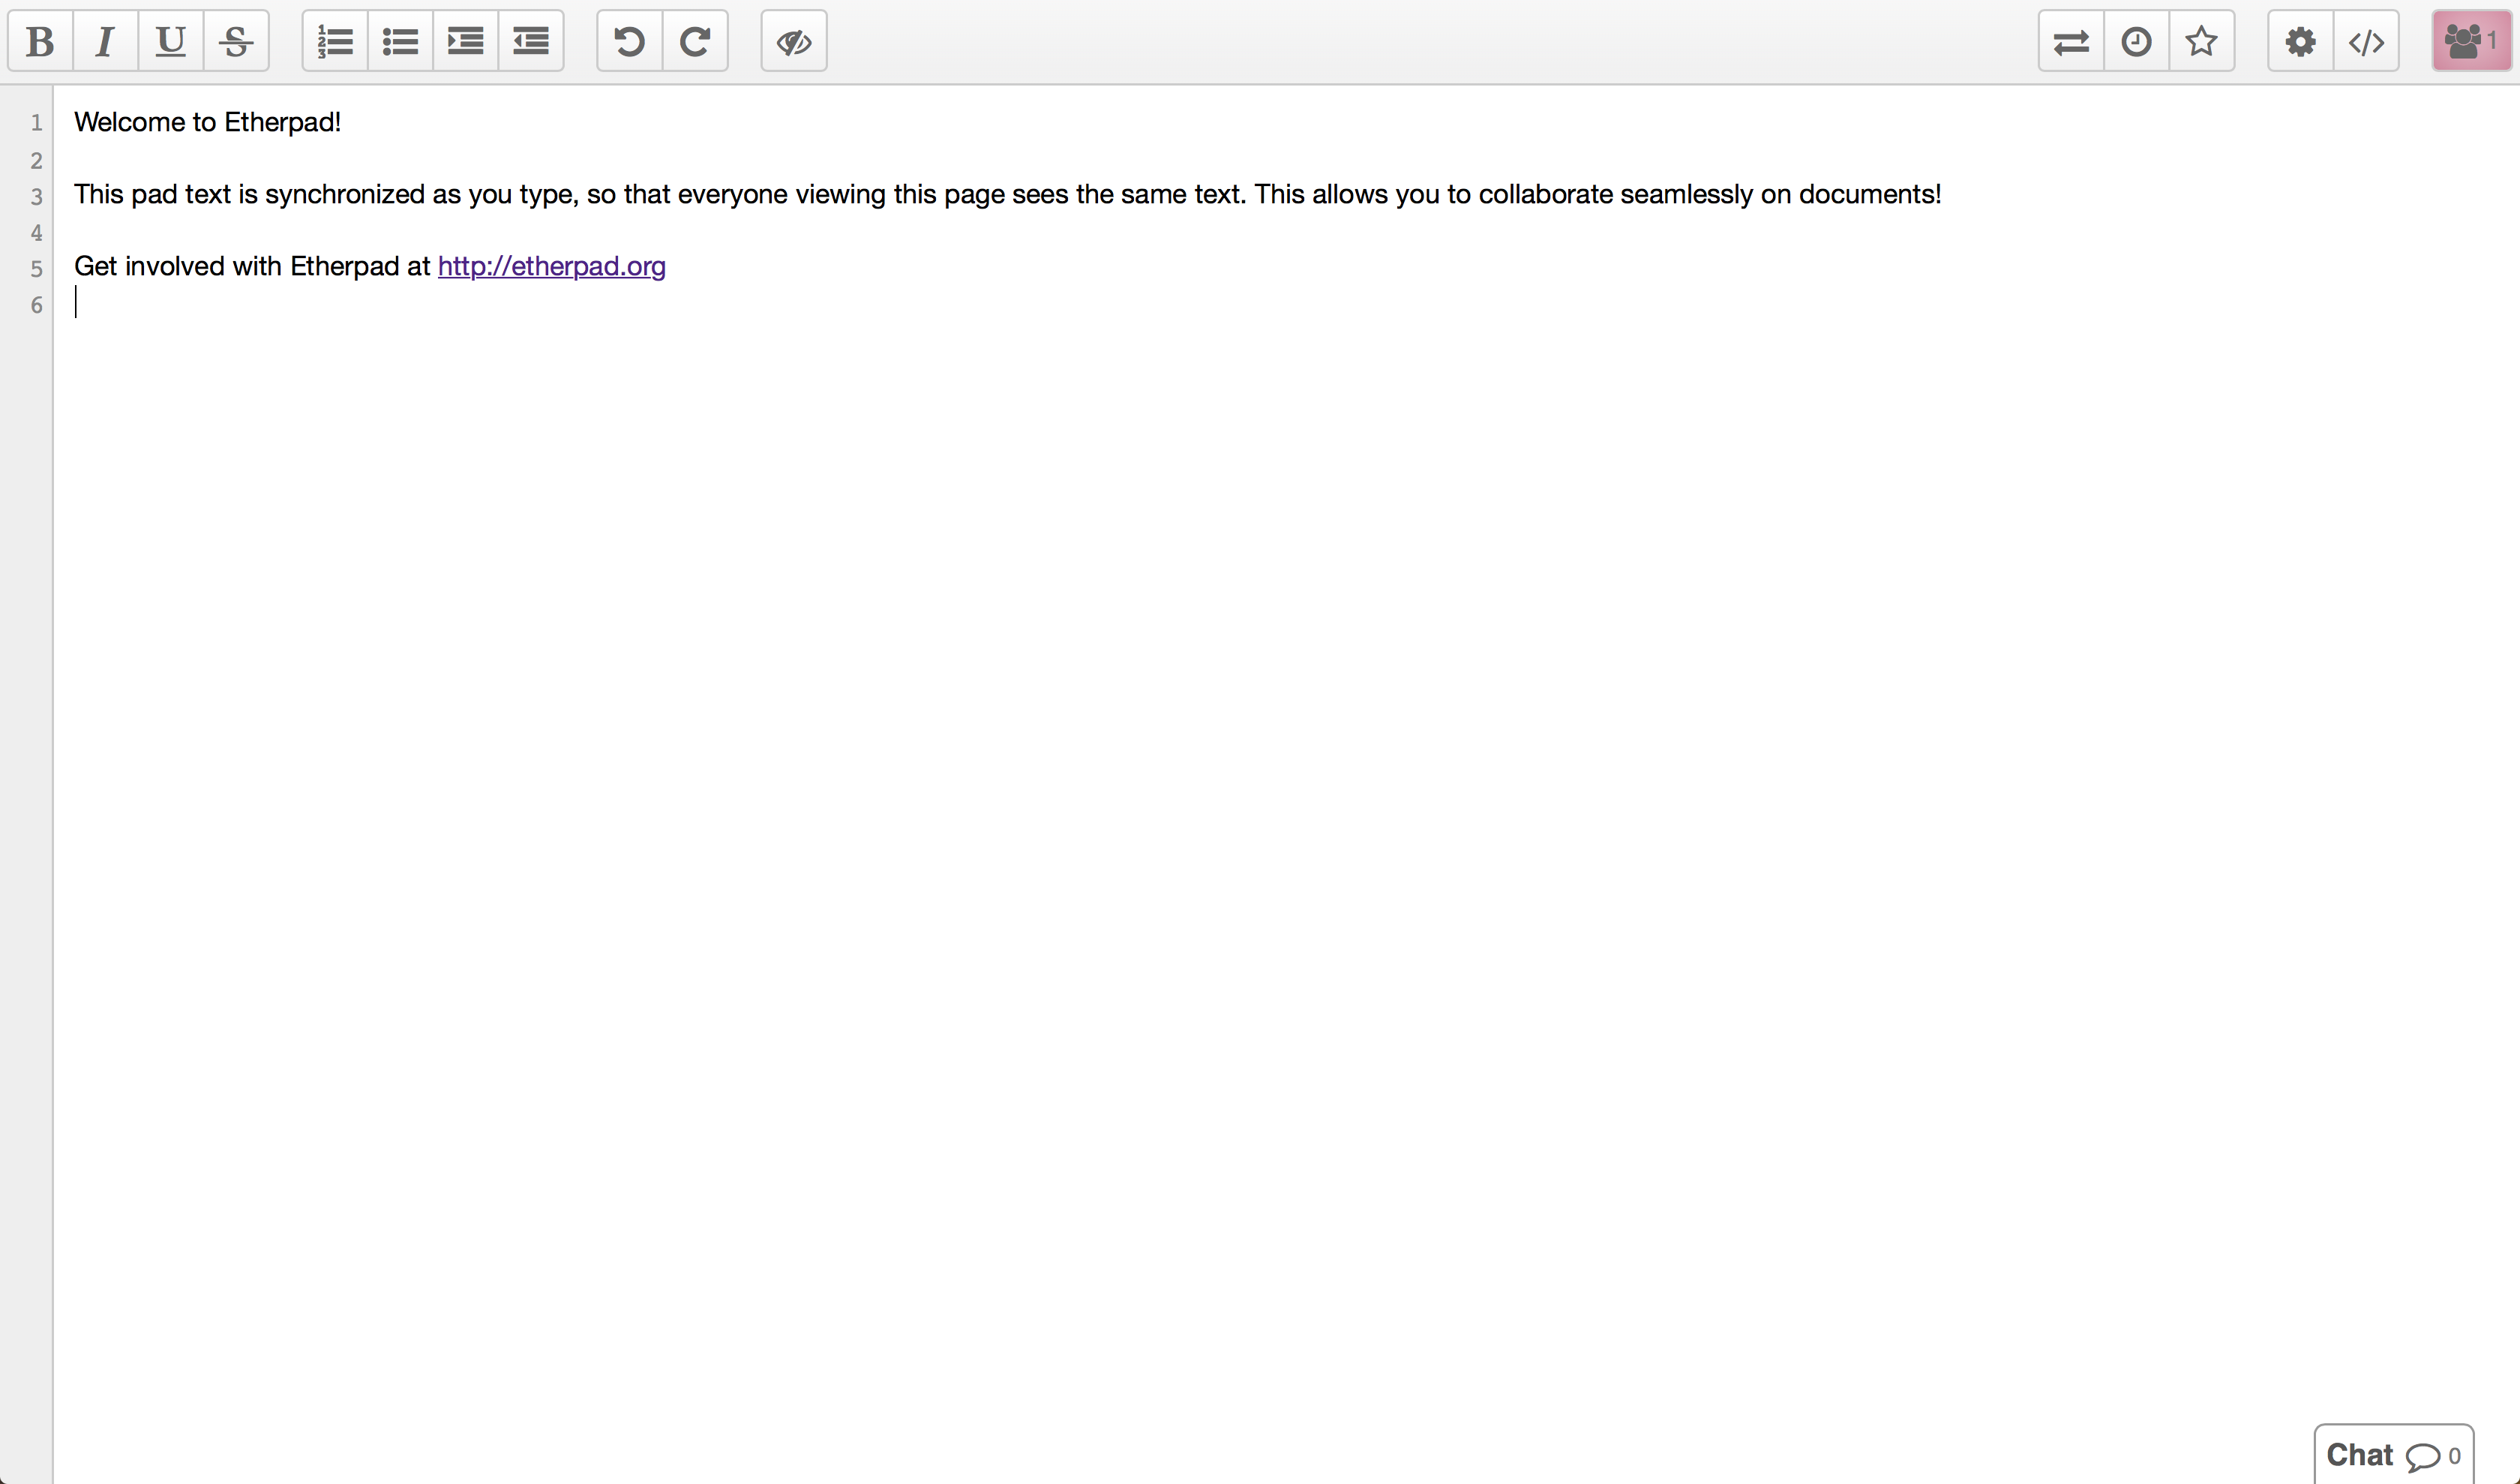
\includegraphics[width=\textwidth]{partials/analyza/etherpad}
    \caption{Ukázka aplikace Etherpad}\label{fig:etherpad}
\end{figure}

\subsection{Codeshare.io}\label{subsec:codeshare.io}

Codeshare.io je textový editor zaměřený na vývojáře a jejich spolupráci ve skutečném čase.
Jako hlavní využití aplikace Codeshare.io její autor zmiňuje pohovory s vývojáři a to díky integrovanému video chatu pomocí technologie \gls{WebRTC}.~\cite{codeshare:home}

\enquote{\textit{Spojil jsem Firebase s Ace editorem a vznikl Codeshare.io, nástroj pro sdílení kódu ve skutečném čase.}}~\cite{codeshare:created} přeložil Jiří Šimeček

Codeshare.io využívá k synchronizaci textu databázi Firebase Real-time Datebase od společnosti Google.
Tato databáze umožňuje jednotlivým klientům naslouchat, kdy se v databázi změní data a následně tyto data načíst.
Jedná se o velmi jednoduchý model synchronizace obsahu na bázi atomických změn a není zde využito žádného pokročilejšího algoritmu pro synchronizaci textu.~\cite{codeshare:created}

\begin{figure}[ht]
    \centering
    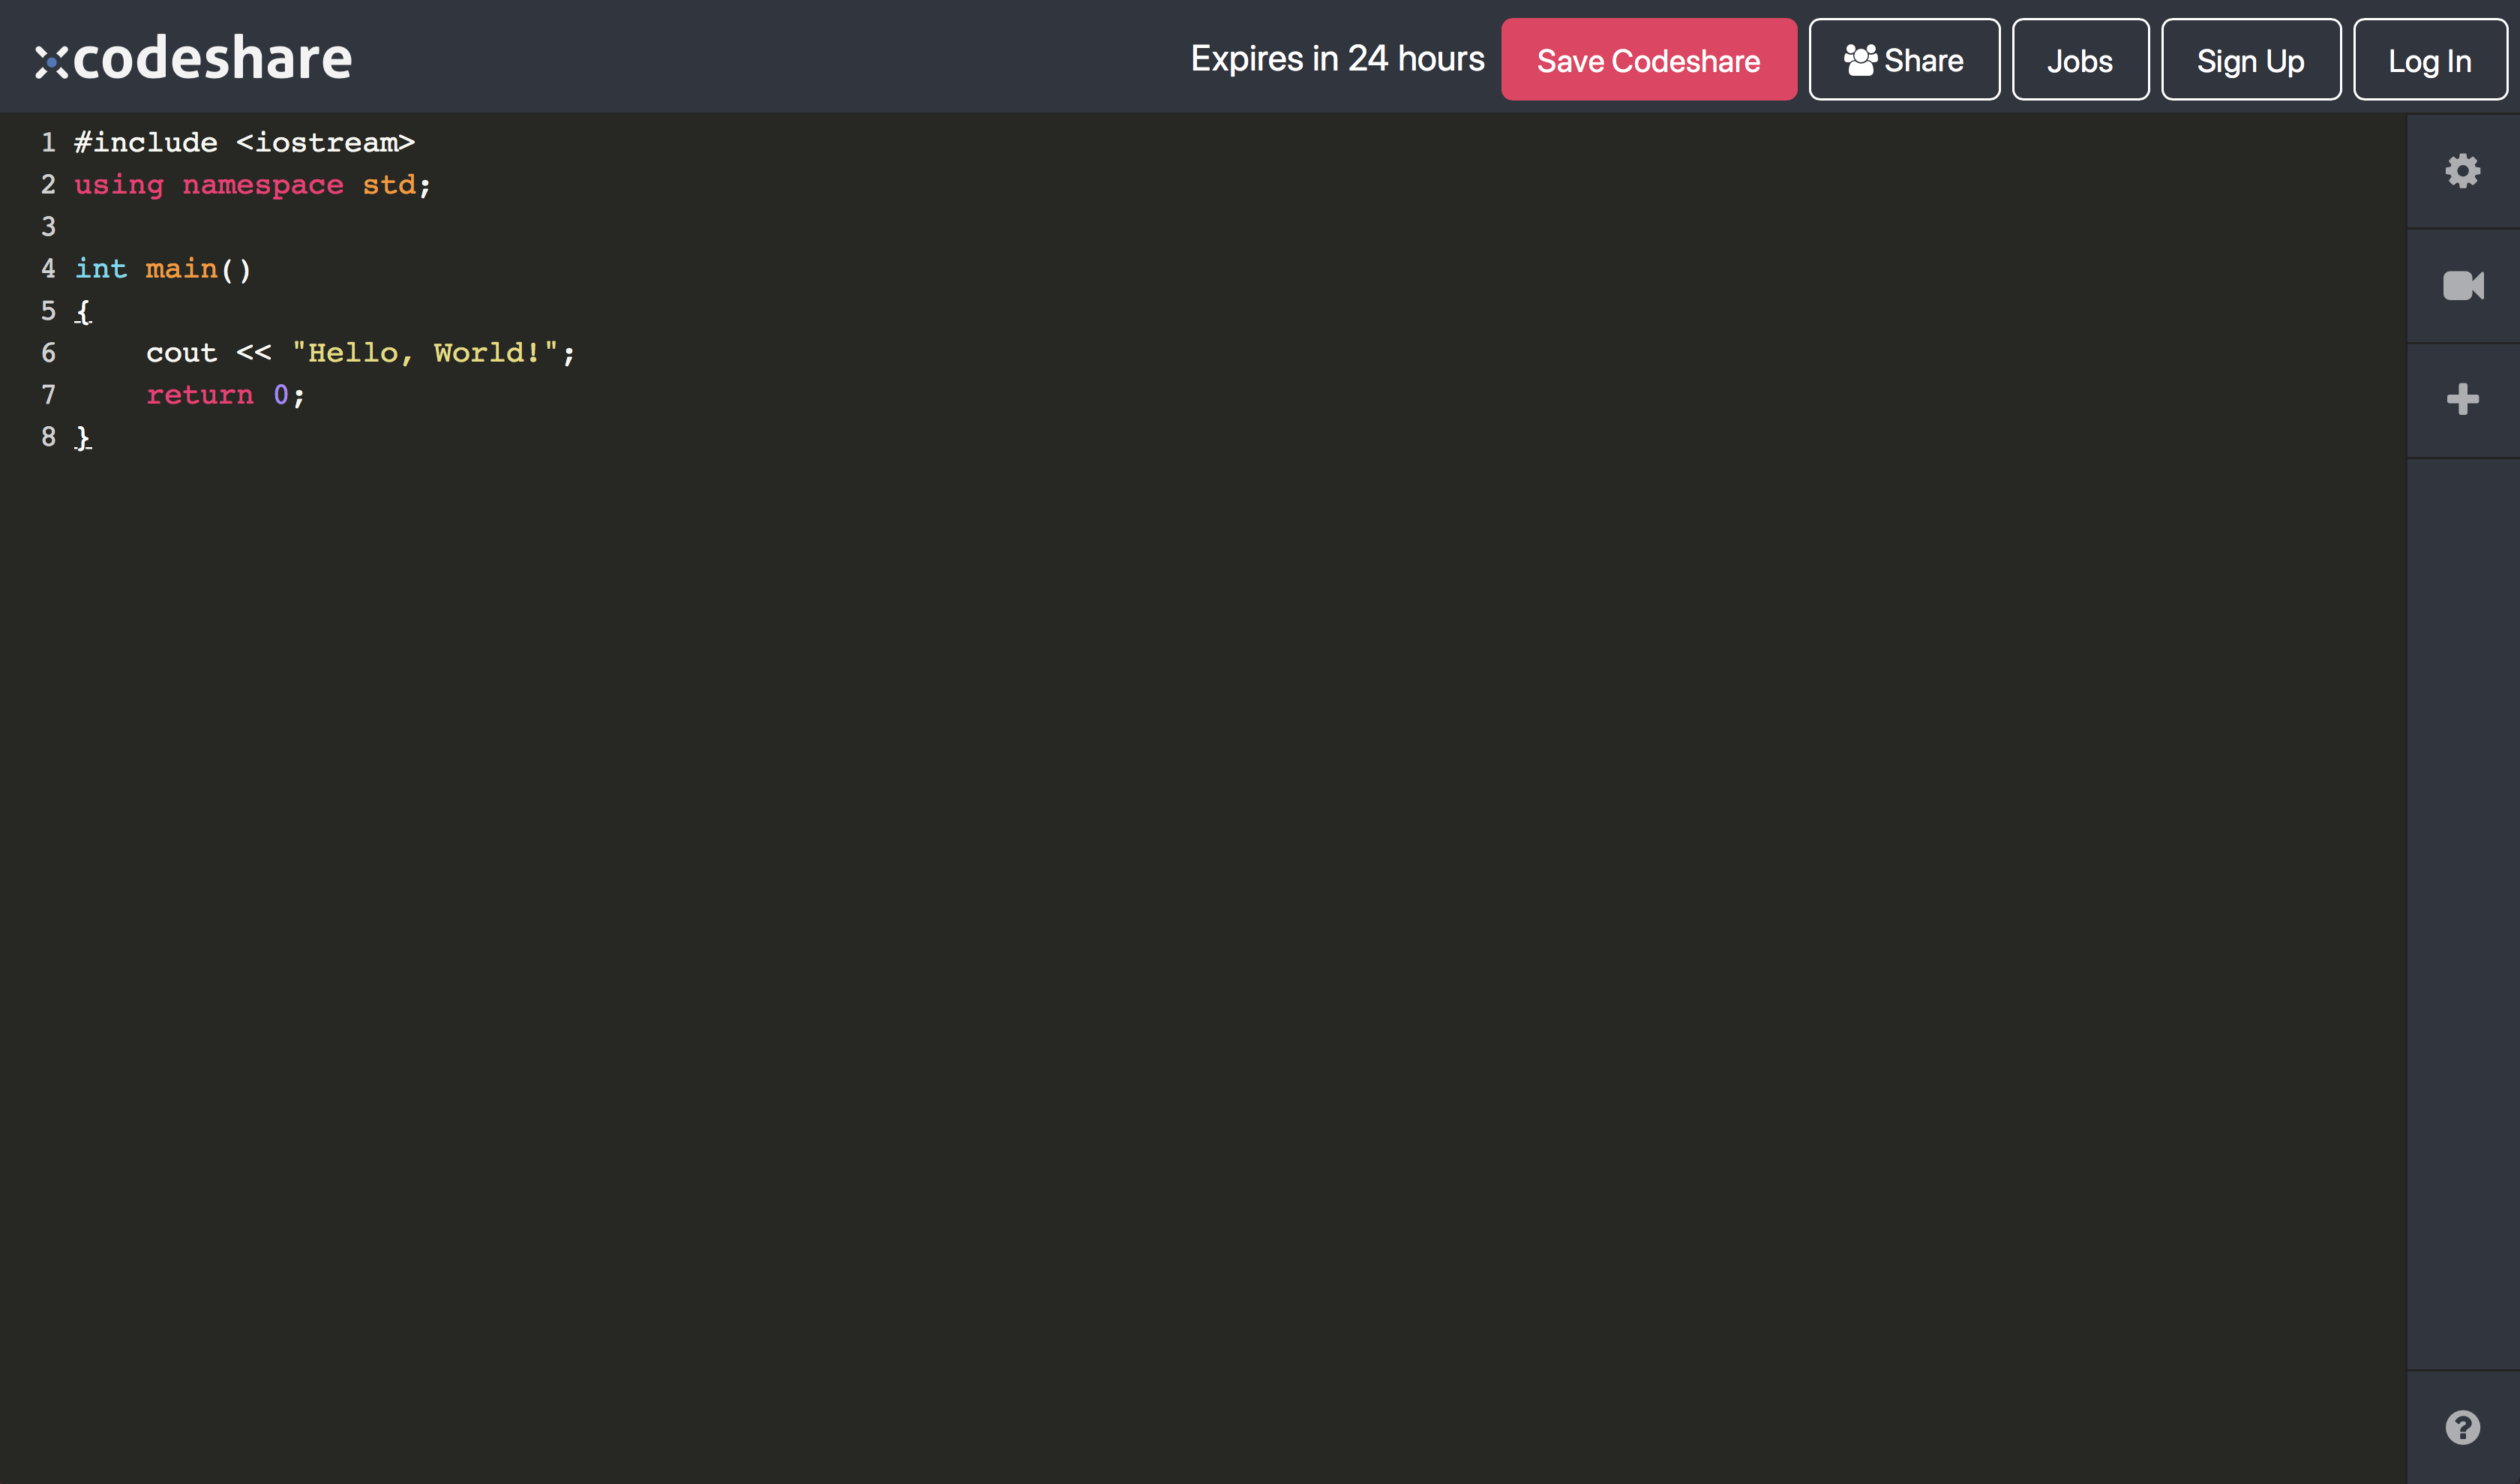
\includegraphics[width=\textwidth]{partials/analyza/codeshare}
    \caption{Ukázka aplikace Codeshare.io}\label{fig:codeshare}
\end{figure}
